\documentclass[12pt, a4paper, oneside, ngerman]{article}

\usepackage{geometry}
\geometry{
	left=3cm,
	right=2cm,
	top=2cm,
	bottom=4cm
}
\usepackage[ngerman]{babel}
\usepackage[utf8]{inputenc}

\usepackage{lmodern}

\usepackage{amsmath}
\usepackage{amsfonts}
\usepackage{amssymb}
\usepackage{graphicx}
\usepackage[final,nopatch=footnote]{microtype}
\usepackage{blindtext}
\usepackage{etoolbox}
\usepackage[pdfborderstyle={/S/U/W 1},hidelinks]{hyperref}
\usepackage{csquotes}
\usepackage{textcomp}
\usepackage{acronym}

\usepackage[onehalfspacing]{setspace}
\usepackage[
    backend=biber,
    style=numeric,
    %style=ieee,
    sorting=none,
  ]{biblatex}
\addbibresource{Literatur.bib}

\usepackage{tabularx}
\usepackage[export]{adjustbox}
\usepackage{blindtext}
\usepackage{epsfig}
\usepackage{longtable}
\usepackage{dcolumn}
\usepackage{here}
\usepackage{floatflt}
\usepackage{dsfont}
\usepackage{graphicx}
\usepackage{epstopdf}
\usepackage[table, svgnames]{xcolor}
\usepackage{listings}
\usepackage{lipsum}
\usepackage{svg}
\usepackage{pdfpages}
\usepackage{lscape}
\usepackage{longtable}
\usepackage{hhline,booktabs}
\usepackage{enumitem}
\usepackage{rotating}
\usepackage{caption}
\usepackage{multirow}
\usepackage{eurosym}

\usepackage[firstpage]{draftwatermark}
\SetWatermarkText{ENTWURF}
\SetWatermarkScale{1}

%JSON-Listing
\usepackage{listings}

\colorlet{punct}{red!60!black}
\definecolor{background}{HTML}{EEEEEE}
\definecolor{delim}{RGB}{20,105,176}
\colorlet{numb}{magenta!60!black}

\usepackage{diagbox}

\lstdefinelanguage{json}{
    basicstyle=\normalfont\ttfamily,
    numbers=left,
    numberstyle=\scriptsize,
    stepnumber=1,
    numbersep=8pt,
    showstringspaces=false,
    breaklines=true,
    frame=lines,
    backgroundcolor=\color{background},
}

\definecolor{gray}{rgb}{0.4,0.4,0.4}
\definecolor{darkblue}{rgb}{0.0,0.0,0.6}
\definecolor{cyan}{rgb}{0.0,0.6,0.6}
\renewcommand{\lstlistingname}{Auflistung}
\lstset{
  basicstyle=\ttfamily,
  columns=fullflexible,
  showstringspaces=false,
  commentstyle=\color{gray}\upshape
}

\lstdefinelanguage{XML}
{
  morestring=[b]",
  morestring=[s]{>}{<},
  morecomment=[s]{<?}{?>},
  stringstyle=\color{black},
  identifierstyle=\color{darkblue},
  keywordstyle=\color{cyan},
  frame=single
  morekeywords={xmlns,version,type,encoding,opcua-servers,server,server_app_uri,client_app_uri,alias,security,policy,mode,server_certificate,client_certificate,client_private_key,nodes,node,DisplayName,NamespaceIndex,IdentifierType,Identifier,datatype,description,modbus-servers,server,ipaddr,port,serveralias,endpoints,endpoint,name,function,address,quantity,offset,type}% list your attributes here
}


\makeatletter
%\renewcommand{\@chapapp}{}% Not necessary...
\newenvironment{chapquote}[2][2em]
  {\setlength{\@tempdima}{#1}%
   \def\chapquote@author{#2}%
   \parshape 1 \@tempdima \dimexpr\textwidth-4\@tempdima\relax%
   \itshape}
  {\par\normalfont\hfill--\ \chapquote@author\hspace*{\@tempdima}\par\bigskip}
\makeatother

\usepackage{tikz}
\newcommand*\circled[1]{\tikz[baseline=(char.base)]{%
            \node[shape=circle,fill=green!80,draw,inner sep=2pt] (char) {#1};}}
\usepackage{enumitem}

\setlength{\parindent}{0em}

\newsavebox{\savefig}


\usepackage{pdfpages}
\setlength\parindent{0pt}

\linespread{1.5}
%\acsetup{first-style=short}    % package acro
\newcounter{SeitenzahlSpeicher}

\begin{document}


%%%%%%%%%%Titelseite%%%%%%%%%%Titelseite%%%%%%%%%%
%%%%%%Titelseite%%%%%Titelseite%%%%%%
%%%%%%Titelseite%%%%%Titelseite%%%%%%
\begin{titlepage}
\begin{center}
\begin{figure}[t]
	
\includegraphics[width=0.6\textwidth, left]{Figures/Logo_HS_Emden_Leer.eps}
\end{figure}

$~~$\\
$~~$\\

{\fontfamily{lmss}\selectfont{\huge {Nuggets of Wisdom: Determining an Upper Limit on the Number Density of Chickens in the Universe}}}\\

\vspace{2cm}

\textbf{Masterarbeit}\\ 
\textbf{im Studiengang Industrial Informatics (M.Eng.)}\\
\textbf{an der Hochschule Emden/Leer}\\

\vspace{1.5cm}

\end{center}
\text{ \hspace{2.5cm} Vorgelegt von:  \hspace{1.0cm}  Carlo Pedersoli, B.Eng.}\\
\text{ \hspace{2.5cm}                 \hspace{3.75cm} Musterstraße 24}\\
\text{ \hspace{2.5cm}                 \hspace{3.75cm} 123456 Musterstadt}\\
\text{ \hspace{2.5cm} Matrikelnummer: \hspace{0.52cm} 654321}\\

\vspace{0.5cm}

\text{ \hspace{2.5cm}1. Gutachter: \hspace{1.31cm} Prof. Dr. rer. nat. Mario Girotti}\\
\text{ \hspace{2.5cm}2. Gutachter: \hspace{1.31cm} Univ.-Prof. Dr.-Ing. Patrick Stewart}\\

\begin{center}

\vspace{1cm}

\text{Hochschule Emden/Leer}\\
\text{Fachbereich Technik}\\

\end{center}	
\end{titlepage}

%%%%%%%%%%Abstract%%%%%%%%%%Abstract%%%%%%%%%%
\pagenumbering{Roman}
\setcounter{page}{1}

%%%%%%%%Sperrvermerk%%%%%Sperrvermerk%%%%%%%%


\begin{center}
    %{\Large \textbf{Sperrvermerk}}
    {\Large \textbf{Erklärung}}
\end{center}
\vspace{.5cm}
%Die vorliegende Arbeit enthält vertrauliche und kommerziell nutzbare Informationen, deren Rechte außerhalb der Hochschule Emden/Leer liegen. Sie darf nur den am Prüfungsverfahren beteiligten Personen zugänglich gemacht werden, die hiermit auf ihre Pflicht zur Vertraulichkeit hingewiesen werden (Sperrvermerk).
Soweit meine Rechte berührt sind, erkläre ich mich einverstanden, dass die vorliegende Arbeit Angehörigen der Hochschule Emden/Leer für Studium, Lehre und Forschung uneingeschränkt zugänglich gemacht werden kann. 

%\newpage
\vspace{2cm}
%%%%%%%%Eigenständigkeitserklärung%%%%%Eigenständigkeitserklärung%%%%%%%%
\begin{center}
    {\Large \textbf{Eigenständigkeitserklärung}}
\end{center}
\vspace{.5cm}
Ich, der Unterzeichnende, erkläre hiermit an Eides statt, dass ich die vorliegende Arbeit selbstständig verfasst habe und keine anderen als die angegebenen Quellen und Hilfsmittel benutzt habe. Alle Quellenangaben und Zitate sind richtig und vollständig wiedergegeben und in den jeweiligen Kapiteln und im Literaturverzeichnis wiedergegeben. Die vorliegende Arbeit wurde nicht in dieser oder einer ähnlichen Form ganz oder in Teilen zur Erlangung eines akademischen Abschlussgrades oder einer anderen Prüfungsleistung eingereicht. Mir ist bekannt, dass falsche Angaben im Zusammenhang mit dieser Erklärung strafrechtlich verfolgt werden können.\newline

\textbf{Einsatz von Künstlicher Intelligenz (KI):}\newline
Im Rahmen dieser Arbeit wurden KI-Anwendungen genutzt, um die sprachliche Konsistenz und Verständlichkeit der Ausführungen zu verbessern, eine einheitliche Ausdrucksweise sicherzustellen sowie zur Unterstützung in der Programmierung der entwickelten Lösungen.
\paragraph{}$~~$\\
\paragraph{}$~~$\\
\vspace{10pt} 
\noindent\rule{5cm}{.4pt}\hfill\rule{5cm}{.4pt}\\%\par
\noindent Ort, Datum \hfill Unterschrift
\newpage

\paragraph{}$~~$\\
\begin{abstract}
\noindent \lipsum[1]
\end{abstract}



\newpage

\paragraph{}$~~$\\
\renewcommand{\abstractname}{Abstract}

\begin{abstract}
\noindent \lipsum[1]
\end{abstract}
\paragraph{}$~~$\\

\begin{chapquote}{Ken Blanchard, \textit{amerikanischer Autor}}
{\Large``None of us is as smart as all of us.''}
\end{chapquote}

\section*{Danksagung}
\lipsum[1]


\newpage
%%%%%%%%Verzeichnisse%%%%%%%%Verzeichnisse%%%%%%%%
%%%%%%%%Inhaltsverzeichnis%%%%%Inhaltsverzeichnis%%%%%%%%
\begin{spacing}{1}
%\pagenumbering{Roman}
%\setcounter{page}{1}
\tableofcontents
\end{spacing}
\newpage

%%%%%%%%Abbildungsverzeichnis%%%%%Abbildungsverzeichnis%%%%%%%%
\begin{spacing}{1}
%\section*{List of figures} 
\addcontentsline{toc}{section}{Abbildungsverzeichnis}
%\renewcommand{\listfigurename}{}
\listoffigures
\addcontentsline{toc}{section}{Quelltextauszüge}
\renewcommand*{\lstlistlistingname}{Quelltextauszüge}
\lstlistoflistings
\end{spacing}
%\newpage

%%%%%%%%Tabellenverzeichnis%%%%%Tabellenverzeichnis%%%%%%%%
%\section*{List of tables} 
\addcontentsline{toc}{section}{Tabellenverzeichnis} 
%\renewcommand{\listtablename}{}
\listoftables
\newpage

%%%%%%%%Abkürzungsverzeichnis%%%%%Abkürzungsverzeichnis%%%%%%%%
\section*{Abkürzungsverzeichnis} 
\addcontentsline{toc}{section}{Abkürzungsverzeichnis}

\begin{acronym}[OPC UA]
\acro{opcua}[OPC UA]{Open Platform Communications Unified Architecture}
\end{acronym}



\newpage

\clearpage
\setcounter{SeitenzahlSpeicher}{\value{page}}
\pagenumbering{arabic}
%%%%%%%%Inhalt%%%%%%%%%%%%%%%%%%%Inhalt%%%%%%%%%%%
\section{Einleitung}\label{sec:S1}

\begin{chapquote}{Stéphane Nappo, \textit{Groupe SEB}}
``One of the main cyber-risks is to think they don’t exist. The other is to try to treat all potential risks.''
\end{chapquote}

Arbeit mit Akronymen: \ac{opcua}\newline

\noindent \lipsum[1-4]


\subsection{Ziel}
\noindent \lipsum[1-2]


\subsection{Motivation}
\noindent \lipsum[1-2]


\subsection{Vorgehen}
\noindent \lipsum[1-2]

\newpage
\section{State of the Art}%\label{sec:S2}

\begin{chapquote}{Stefan Hoppe, \textit{Präsident OPC Foundation}}
``Protokolle werden immer unwichtiger - es geht immer um den sicheren Austausch von standardisierten Informationen.''
\end{chapquote}

\noindent \lipsum[1-2]

\subsection{Lorem ipsum}
\noindent \lipsum[1-2]

\begin{figure}[h]
    \centering
    
\includegraphics[width=1.0\linewidth]{Figures/Platzhalter.png}
    \caption{Genereller Aufbau eines Automatisierungssystems nach Lauber \cite{Lauber1999}.}
    \label{fig:Prozessautomatisierungssystem}
\end{figure}

\noindent \lipsum[1-2]

\subsection{Lorem ipsum svg}
\noindent \lipsum[1-4]
\begin{figure}%[h]
  \centering
  \includesvg[width=\linewidth, inkscapelatex=false]{Figures/Timeline.svg}
  \caption{Zeitliche Einordnung identifizierter Malware-Angriffe auf OT-Systeme}
  \label{fig:Timeline}
\end{figure}


\newpage
\section{Anforderungen}\label{sec:S3_RQ}
\noindent \lipsum[1]

% https://tex.stackexchange.com/questions/280462/link-to-arbitrary-part-of-text
%\texorpdfstring{\protect\hyperlink{mylink}{As shown here}}{}\newline
%\hyperlink{mylink}{As shown here}\\
%\hypertarget{mylink}{\textbf{Here is the anchor}}

\subsection{Funktionale Anforderungen}
Die funktionalen Anforderungen definieren das gewünschte Verhalten des Systems im Hinblick auf Kommunikation, Datenverarbeitung und Interaktion (...). Zur besseren Übersicht werden die funktionalen Anforderungen im Folgenden mit \textbf{RQ-F} abgekürzt. Die Abkürzung dient der fortlaufenden Nummerierung und ermöglicht eine eindeutige Referenzierung dieser Anforderungen in den folgenden Kapiteln.
\subsubsection{Kommunikations- und Systemverhalten}
\hypertarget{RQ-F-01}{\textbf{RQ-F-01 – Lorem ipsum}}\newline
\noindent \lipsum[1]\newline

%{\color{red}
\hypertarget{RQ-F-02}{\textbf{RQ-F-02 – Lorem ipsum}}\newline
\noindent \lipsum[1]\newline

\subsection{Nicht-funktionale Anforderungen}
Nicht-funktionale Anforderungen legen qualitative Eigenschaften des Systems fest, wie Sicherheit, Interoperabilität und Echtzeitfähigkeit. Sie betreffen das Wie der Umsetzung und stellen sicher, dass das System zuverlässig, flexibel und in bestehende Infrastrukturen integrierbar ist. Analog zu den funktionalen Anforderungen werden nicht-funktionale Anforderungen mit \textbf{RQ-NF} abgekürzt und fortlaufend nummeriert.
\subsubsection{Sicherheit}
\hypertarget{RQ-NF-01}{\textbf{RQ-NF-01 – Lorem ipsum}}\newline
\noindent \lipsum[1]\newline

\hypertarget{RQ-NF-02}{\textbf{RQ-NF-02 – Lorem ipsum}}\newline
\noindent \lipsum[1]\newline

\section{Entwicklung und Realisierung}\label{sec:S4}
\lipsum[1-2] \footnote{\url{https://www.google.com}}

\subsection{Lorem ipsum}
\lipsum[1-4]

\subsection{Lorem ipsum}
\lipsum[1-4]
\newpage
\section{Evaluierung}\label{sec:Evaluation}

\begin{chapquote}{James Langevin, \textit{ehem. Mitglied des US-Repräsentantenhauses}}
``Effective cybersecurity is not a product, but a process.''
\end{chapquote}

\lipsum[1-4]

\subsection{Abschließende Bewertung der Evaluierung}
\lipsum[1-2]
\newpage
\section{Fazit}\label{sec:S7}
\lipsum[1-4]

\newpage
\section{Ausblick}\label{sec:ausblick}

\begin{chapquote}{James Scott, \textit{Institute for Critical Infrastructure Technology}}
``There’s no silver bullet solution with cyber security, a layered defense is the only viable defense.''
\end{chapquote}

\lipsum[1-4]
\clearpage



%%%%%%%%Literaturverzeichnis%%%%%Literaturverzeichnis%%%%%%%%
\setcounter{biburllcpenalty}{7000}
\setcounter{biburlucpenalty}{8000}
\printbibliography[heading=bibintoc]
\newpage
\clearpage

%%%%%%%%Anhang%%%%%Anhang%%%%%%%%
%\pagenumbering{Roman}
%\pagenumbering{gobble}
\appendix

\section{Appendix}
%\subsection{Anhang A1}\label{sec:A1}
%\includepdf[pages=-]{Anhang/NE177_Requirements.pdf}
\subsection{Malware-Angriffe auf Automatisierungssysteme}\label{sec:A_Malware_Tabelle}


%\begin{landscape}
\begin{table}[H]
\centering
\rotatebox{90}{
\resizebox{1\textwidth}{!}{%\begin{minipage}{2\textwidth}%
\begin{tabular}{|l|l|l|l|l|c|}
\hline
 \rowcolor{FireBrick!80}
\textbf{Jahr} & \textbf{Ort} &\textbf{ Malware/Name} & \textbf{Details des Events} & \textbf{Angriffsart} & \textbf{Literatur} \\ \hline
2010 & Iran & Stuxnet & \begin{tabular}[c]{@{}l@{}}Infiltration von Programmier-\\ geräten (PG) und Zerstörung \\ von Zentrifugen durch \\ Steuerungsmanipulation\end{tabular} & \begin{tabular}[c]{@{}l@{}}Infiltration von PGs über infizierte\\ USB-Sticks, Injektion von schad-\\ haftem Step7 Funktionscode in \\ Siemens S7-300 Steuerungen und \\ Manipulation der Kommunikation \\ mit den Zentrifugen\end{tabular} & \cite{Symantec_Stuxnet} \\ \hline
2015/2016 & Ukraine & \begin{tabular}[c]{@{}l@{}}Crashoverride/\\ Industroyer\end{tabular} & \begin{tabular}[c]{@{}l@{}}Blackout durch einen Denial-\\ of-Service-Angriff auf Steuer-\\ ungen und SCADA-Systeme\end{tabular} & \begin{tabular}[c]{@{}l@{}}Angriff auf SPS- und SCADA-\\ Systeme des Übertragungs-\\ netzes mit den OT-Protokollen \\ IEC-101, IEC-104, IEC-61850 \\ und OPC-DA\end{tabular} & \cite{Cashoverride_Dragos} \\ \hline
2017 & Mittlerer Osten & Triton/TRISIS & \begin{tabular}[c]{@{}l@{}}Versuchte Remote-Übernahme\\ der Steuerung einer petro-\\ chemischen Anlage\end{tabular} & \begin{tabular}[c]{@{}l@{}}Angriff auf Schneider Electric \\ Triconex Sicherheitssysteme\\ (Safety Instrumented Systems,\\ SIS) und Injektion von schad-\\ haftem Steuerungscode (KOP)\end{tabular} & \cite{TRISIS_Dragos} \\ \hline
2022 & Ukraine & \begin{tabular}[c]{@{}l@{}}Industroyer2 + \\ INCONTROLLER/\\ PIPEDREAM\end{tabular} & \begin{tabular}[c]{@{}l@{}}Versuchter DoS-Angriff auf \\ das Energienetz und System-\\ Infiltration über unsicheres \\ OT-Equipment\end{tabular} & \begin{tabular}[c]{@{}l@{}}Angriff auf SPS/SCADA über \\ das IEC-104 OT-Protokoll,\\  Infiltration von OT-Kom-\\ ponenten (Siemens, Schneider \\ Electric, Omron, etc.) über \\ Netzwerk-Protokolle wie OPC\\ UA, MODBUS, CODESYS,\\ Machine Expert und Omron \\ FINS\end{tabular} & \cite{Industroyer2_forescout} \\ \hline
2022 &  & PIPEDREAM & \begin{tabular}[c]{@{}l@{}}Entdeckung der ICS-Malware\\ PIPEDREAM\end{tabular} & \begin{tabular}[c]{@{}l@{}}Infiltration von IT- und OT-\\ Netzwerken, Manipulation \\ von OPC UA Servern sowie \\ Steuerungen von Omron und \\ Schneider Electric über \\ MODBUS und CODESYS-\\ Schnittstellen\end{tabular} & \cite{Pipedream_Dragos} \\ \hline
\end{tabular}%
%\caption{Übersicht identifizierter Malware-Angriffe auf OT-Systeme in den vergangenen Jahren.}
%\end{minipage}
}}
\caption{Übersicht identifizierter Malware-Angriffe auf OT-Systeme in den vergangenen Jahren.}
%}
\label{tab:Tabelle_1}
%}
\end{table}
%\end{landscape}

\clearpage

\subsection{XML-Konfigurationsdatei}\label{sec:A1}
\subsubsection{Auzug aus einer XML}
\begin{lstlisting}[language=XML, frame=single, caption={Lorem ipsum.}, label={lst:xml-label}, captionpos=b]
<?xml version="1.0" encoding="UTF-8"?>
<opcua-servers xmlns:xsi="http://www.w3.org/2001/XMLSchema-instance"
               xsi:noNamespaceSchemaLocation="opcua-endpoints.xsd">

  <server>
    <server_app_uri>opc.tcp://172.16.4.52:4840</server_app_uri>
    <client_app_uri>urn:omag:demonstrator</client_app_uri>
    <alias>unsecured-revpi-opcua-server</alias>
    <security>
      <policy>SecurityPolicyNone</policy>
      <mode>None</mode>
    </security>
    <nodes>
      <node>
        <DisplayName>Produzierte_Takte</DisplayName>
        <NamespaceIndex>3</NamespaceIndex>
        <IdentifierType>Numeric</IdentifierType>
        <Identifier>9</Identifier>
        <datatype>String</datatype>
        <description>Names of available files</description>
      </node>
    </nodes>
  </server>
  
</opcua-servers>
\end{lstlisting}
\newpage

\subsection{Secure IoT Gateway in der Digitalen Fabrik}\label{sec:A_Demonstrator}
\begin{figure}[H]
    \centering
    \savebox{\savefig}{
\includegraphics[width=1.35\linewidth]{Figures/Platzhalter.png}}
    \rotatebox{90}{%
        \begin{minipage}{\wd\savefig}
            \usebox{\savefig}
            \caption{Lorem ipsum ...}
            \label{fig:Anhang_Demonstrator_Topview}
        \end{minipage}}
\end{figure}

\begin{figure}[H]
    \centering
    \savebox{\savefig}{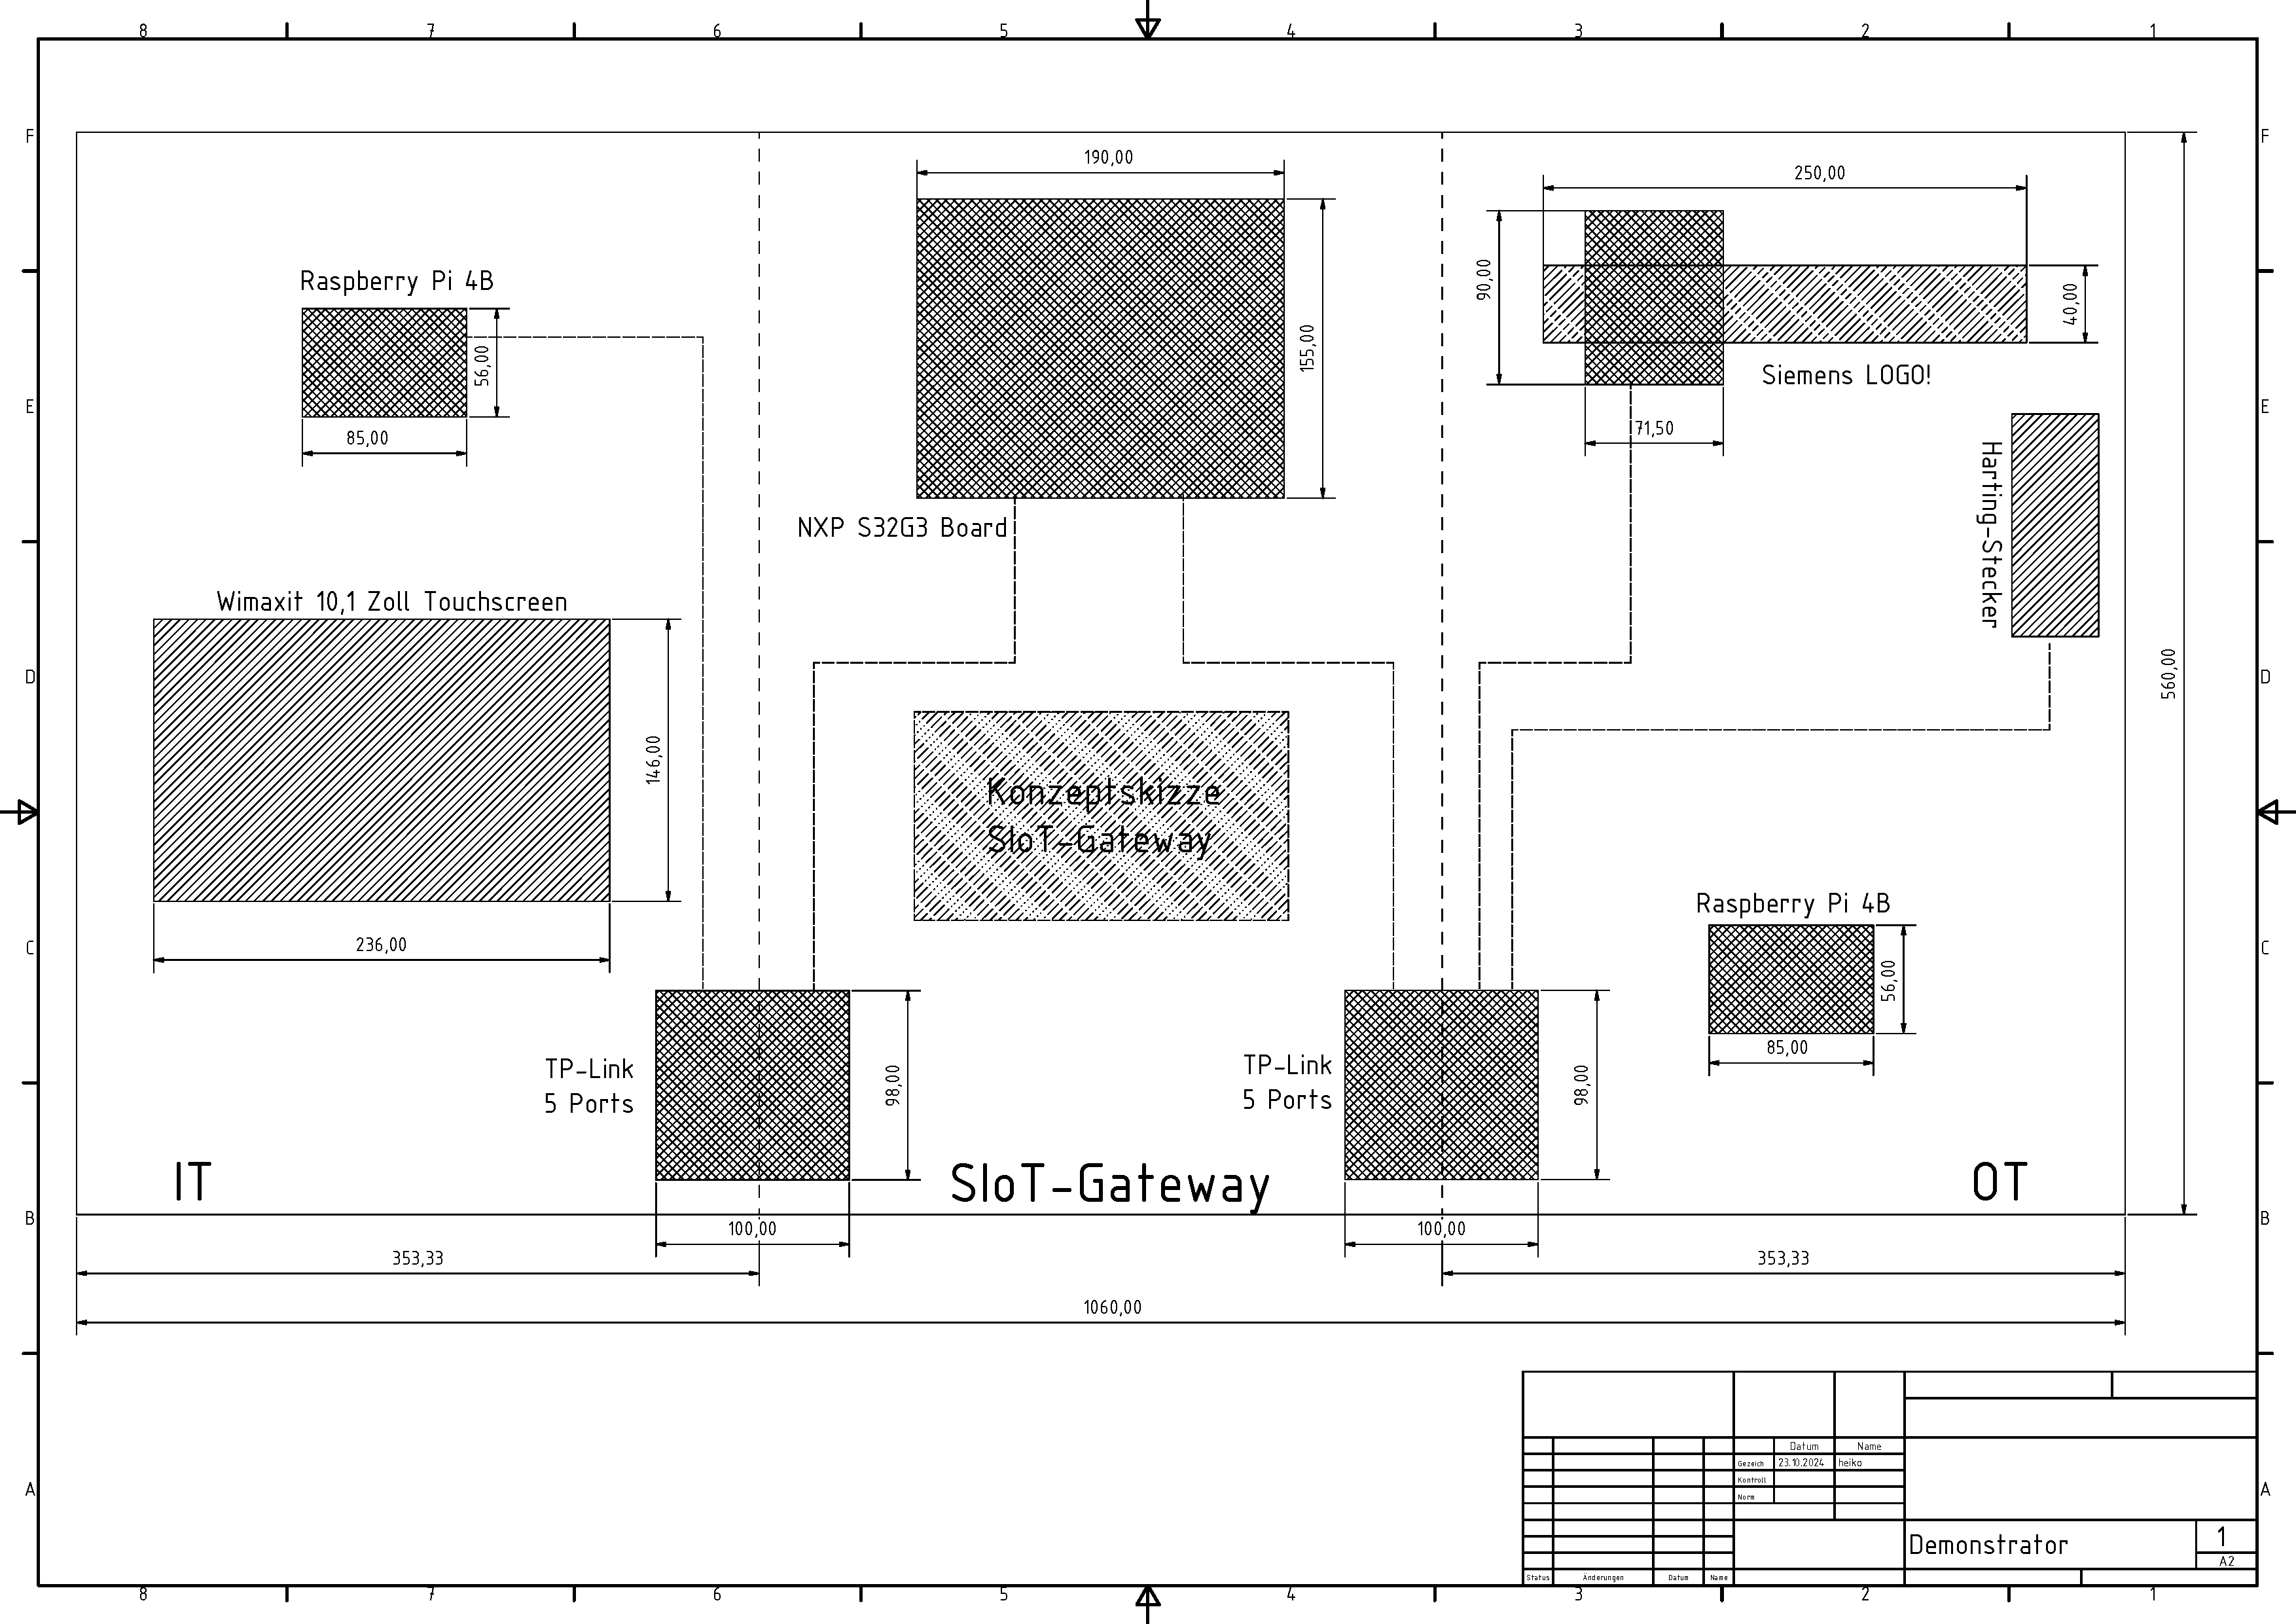
\includegraphics[width=1.3\linewidth]{Anhang/Demonstrator.pdf}}
    \rotatebox{90}{%
        \begin{minipage}{\wd\savefig}
            \usebox{\savefig}
            \caption{Lorem ipsum... (vgl. Abb. \ref{fig:Anhang_Demonstrator_Topview}).}
            \label{fig:Demonstrator}
        \end{minipage}}
\end{figure}
\newpage

%\subsection{A1}\label{sec:A1}
% ...
%\includepdf[pages=-]{Anhang/Angebot_Harting_Stecker.pdf}

%\subsection{A2}\label{sec:A2}
% ...
%\includepdf[pages=-]{Anhang/Dokumentation_Harting-Industriestecker.pdf}

\end{document}